%%%%%%%%%%%%%%%%%%%%%%%%%%%%%%%%%%%%%%%%%
% University Assignment Title Page 
% LaTeX Template
% Version 1.0 (27/12/12)
%
% This template has been downloaded from:
% http://www.LaTeXTemplates.com
%
% Original author:
% WikiBooks (http://en.wikibooks.org/wiki/LaTeX/Title_Creation)
%
% License:
% CC BY-NC-SA 3.0 (http://creativecommons.org/licenses/by-nc-sa/3.0/)
% 
% Modified for COSC480/490 by:
% Lech Szymanski (8/3/18)

\documentclass[12pt]{article}
\usepackage[draft]{cosc4x0style}
\usepackage[ruled, linesnumbered,lined]{algorithm2e}
\usepackage{amsmath}
\usepackage{amssymb}
\usepackage{breakcites}
\usepackage{color}
\usepackage{caption}
\usepackage[linguistics]{forest}
\usepackage{marginnote}
\usepackage{todonotes}
\usepackage{subcaption}
\usepackage{rotating}
\usepackage{url}

% Code listings styles %
\usepackage{listings}
\usepackage{xcolor}
 
\definecolor{codegreen}{rgb}{0,0.6,0}
\definecolor{codegray}{rgb}{0.5,0.5,0.5}
\definecolor{codepurple}{rgb}{0.58,0,0.82}
 
\lstdefinestyle{mystyle}{
    commentstyle=\color{codegreen},
    keywordstyle=\color{magenta},
    numberstyle=\tiny\color{codegray},
    stringstyle=\color{codepurple},
    basicstyle=\ttfamily\footnotesize,
    breakatwhitespace=false,         
    breaklines=true,                 
    captionpos=b,                    
    keepspaces=true,                 
    numbers=left,                    
    numbersep=5pt,                  
    showspaces=false,                
    showstringspaces=false,
    showtabs=false,                  
    tabsize=2
}
 
\lstset{style=mystyle}

\newcommand{\keyword}[1]{%
    \textbf{#1}%
    % Add keyword to the margin
    % \todo[color=none, linecolor=none]{#1}%
}

\usepackage[round]{natbib}   % omit 'round' option if you prefer square brackets
\bibliographystyle{plainnat}
% \bibliographystyle{apalike}
% \usepackage[usenames,dvipsnames,svgnames,table]{xcolor}

% To compile the final version of the report (which will remove all the todo content)
%\usepackage{cosc4x0style}

% Specify project code 480 or 490
\papercode{480}

% Your project title
\title{Quantifying Conceptual Density in Text}

% Your name
\author{Anthony \textsc{Dickson}}
\studentid{3348967}

% Names of your supervisors, separated by line break '\\'
\supervisors{
  Anthony \textsc{Robins} \\
  Alistair \textsc{Knott}
}

% Date, change the \today to a set date if you want to be precise
\reportdate{\today}

\begin{document}
\maketitle

\begin{abstract}
In introductory programming courses across many institutions, educators have observed an unusually high rate of both fail and high grades. One explanation for the cause of this phenomenon mentions the idea that concepts within programming languages are tightly integrated, perhaps more so than some other disciplines. In domains of tightly integrated concepts, learning a concept depends greatly on the successful learning of the prerequisite concepts. As such, learning outcomes tend to be self-reinforcing; successful learning promotes further successful learning and unsuccessful learning promotes further unsuccessful learning. This idea of a domain of concepts being tightly integrated is referred to as conceptual density.
% Conceptual density is theorised to be a large factor in learning difficulty, and subsequently successful learning. 
% To the best of my knowledge, no method for quantifying conceptual density exists in the current literature. 
In this report I set out to define conceptual density with reference to cognitive load theory, and develop a method for quantifying conceptual density in well-structured expository text documents using natural language processing methods and graph analysis techniques.
\end{abstract}

\tableofcontents
\clearpage

\section{Introduction}
It is thought that the unusually high rate of fail and high grades observed in introductory programming courses is possibly due to concepts in programming languages being unusually tightly integrated \citep{robins2010learning}. A tightly integrated concept is a concept that is difficult to describe independently of other concepts. Tightly integrated concepts are said to magnify the effects of learning edge momentum and lead to the polarised outcomes observed in introductory programming courses. This report is interested in conceptual density, a sort of measure concerned with the level of integration for concepts in a given domain.  

The notion of this idea of conceptual density affecting learning difficulty is not unique to the aforementioned work. It appears in the literature on cognitive load theory, in a perhaps slightly different form, as the ``element interactivity effect'', which says that the number of interacting elements in a task is the main contributor to cognitive load - a measure of mental exertion required to perform a given task \citep{sweller1994cognitive}. Cognitive load theory provides an explanation of aspects of learning difficulty and can be used to guide education and instructional design.

To the best of my knowledge there exists no objective measure in the current literature of the element interactivity effect, or the notion of conceptual density. Element interactivity appears to be estimated manually and it depends greatly on the knowledge of the learner \citep{chandler1996cognitive}, and as such remains subjective. In \citep{robins2010learning} the notion of concepts being tightly integrated stems from the observation that educators typically fail to reach a consensus on how to structure introductory programming courses (this is supposedly not the case in other disciplines).  While no measure of conceptual density was clearly defined in that work, some possible ways to do so were proposed.

In this report,  I follow up on the notion of conceptual density and set out to elaborate on its definition and develop an objective measure of conceptual density in the context of well-structured expository text documents (e.g. textbooks, scientific papers). For measuring conceptual density I explore one of the methods mentioned in \citep{robins2010learning} - analysing a mind-map like graph structure. Whereas in the original work, this approach was suggested as a characterisation of  introductory programming course material to be generated by experts, in this report I aim to build up and analyse mind-map like graph structures automatically and systematically through the use of natural language processing methods and graph analysis techniques.

The proposed method will be evaluated first through experiments using small hand-crafted text documents and then on a selection of expository text documents. The end goal of this report is to be able to systematically generate scores of conceptual density that are objective and in line with human judgements. Ideally, the scores would be able to be used to compare text documents and also identify which sections in a given text are conceptually dense.

% Some domains of knowledge are structured in ways that inhibit learning and understanding, and some in ways that promote learning and understanding. One indicator of how difficult a domain may be to understand or learn is the element interactivity effect \citep{sweller2011element}. It is said that the number of elements in a domain and the degree to which they interact is an indicator of how much cognitive load may be imposed on one trying to understand the domain. Element interactivity, and by extension the overall cognitive load, of a given task is a function of extraneous cognitive load and intrinsic cognitive load. Extraneous cognitive load deals with learning difficulty imposed by the manner in which the task is presented (instructional design). On the other hand, intrinsic cognitive load is about the learning difficultly that is inherent to a task, regardless of how the task is represented.
% %  Under Cognitive Load Theory, it is thought that an individual has a limited amount of cognitive resources, and when operating near or at maximum capacity (i.e. high cognitive load) learning is significantly inhibited.

% We introduce the idea of conceptual density with the element interactivity effect at its core to help measure the learning difficulty of a domain. We look at measuring conceptual density in text documents, in particular well-structured expository documents such as textbooks and scientific research papers. We use a combination of natural language processing methods and graph analysis methods to synthesise a model to quantify conceptual density. We first test our model on a small hand-crafted corpus before testing the model on a selection of textbooks and research papers.

% The proposed approach is to create a graph structure that encodes the concepts present in a text document and the relationships between them, and to analyse the graph topology to generate a scoring of conceptual density. This score can then be used to compare two documents to see which one is more conceptually dense. Also, the generated graph structure can be used to further identify important/central concepts and interesting portions of the text.

\section{Background}
\subsection{Learning Edge Momentum}
% \todo[inline]{Need to actually read the paper again and make sure what I've said is correct!}
% Another theory on learning is that we learn at the edges of our knowledge \citep{robins2010learning}.
% One of the main concerns of this paper is that a bad learning experience may lead to bad momentum that hinders further learning, whereas a good learning experience may be self-reinforcing leading to good momentum that benefits further learning. This could provide insight to how the way a text document, or more generally a domain of knowledge, is constructed could affect ones ability to assimilate knowledge from it. For example, some concepts in a text may be introduced before they are fully explained and acquired by a learner, forcing them to `p' the referenced idea until it is explained fully later on.
Learning edge momentum was proposed as an explanation for the unusually high rate of both fail and high grades in introductory computer science courses \citep{robins2010learning}. The hypothesis builds upon the idea that we learn at the edges of what we know - it is easy to learn things that build upon what we already know. The core of the hypothesis is that learning outcomes are self-reinforcing; successful learning helps further successful learning of closely related concepts, and unsuccessful learning tends to lead to further unsuccessful learning of closely related concepts. With successful learning one builds up positive momentum and with unsuccessful learning one builds up negative momentum. It is said that concepts in programming languages tend to be tightly integrated, that concepts are difficult to describe or understand independently of each other. This means that learning a new concept is greatly dependent on the understanding of the prerequisite concepts. And because of this the effects of learning edge momentum in introductory programming courses are particularly pronounced, leading to the polarised distribution of grades. 

Conceptual density (as it is defined in this report) was mentioned in this paper as a possible way of providing more concrete evidence to educators on how to structure an introductory computer science curriculum. Mind maps are suggested as a way of representing the material in a course. Here we represent the domain of concepts as a graph structure, where the concepts present in the material are represented with a node in the graph and edges between nodes represent a connection between concepts. This follows the main ideas behind semantic networks and knowledge graphs \citep{sowa1987semantic, zhang2002knowledge, koncel2019text}, an area of research concerning knowledge representation using graphs. This idea of a mind map of concepts forms the basis for the work in this paper.

\subsection{Cognitive Load Theory}
Cognitive load theory provides a framework about learning difficulty and instructional design \citep{sweller1994cognitive}. In CLT (cognitive load theory) the main task of the brain is characterised as information processing, and each person has a certain amount of working memory to process information. Performing tasks requires an amount of mental exertion and concentration, called cognitive load. When the amount of cognitive load exceeds the capacity of an individual's working memory, performing the given task becomes much more difficult. 

If we are to explain this by analogy, the idea of working memory is similar in some ways to computer RAM and running out of working memory is akin to what happens when a computer runs out of RAM. When a computer runs out of RAM, it starts thrashing and all of the programs will become very slow and take many times longer to run compared to when there is enough RAM. By reducing the number of programs that are running we can reduce the memory usage and prevent the computer from thrashing. Similarly, under CLT we can reduce cognitive load by reducing the number of things that must be considered simultaneously to perform a given task in order to make it easier to perform that task. 

The main contributor to the difficulty of a task is number of things that must be considered simultaneously and the degree to which they interact. In CLT this idea is captured by the \keyword{element interactivity effect} \citep{sweller2011element}. The cognitive load imposed by element interactivity is said to be intrinsic to the material itself (\keyword{intrinsic cognitive load}), meaning that no matter how you present that material there will be a certain level of difficulty.

How we present material can affect how difficult it is understand it. For example, consider trying to teach beginner programmers what all of the keywords mean in a Java program that simply prints a message to the screen (see Figure \ref{fig:java_hello_world}) and what each part of the code does. This would likely be too much to learn at once. Here there are many interacting elements (e.g. access modifiers, classes, types, functions, function arguments, comments, member fields, member functions, function calls, string literals) just in this simple program. Instructors typically make these initial lessons easier to follow by giving a simplified, high-level explanation and omitting details that are deemed unnecessary to know at that given point in the course. Changing how the material is presented has the effect of increasing or reducing \keyword{extraneous cognitive load}, cognitive load that is not intrinsic to the material itself but to how it is presented. 

\begin{figure}
    \centering
     \lstset{xleftmargin=20pt}
    \lstinputlisting[language=Java]{docs/HelloWorld.java}
    \caption{Java hello world example}
    \label{fig:java_hello_world}
\end{figure}

Once they have practised Java programming more and have learned the fundamentals well, the details can be learned more easily. This is because the learner will be more familiar with the fundamental ideas, and performing tasks with these ideas is easier due to their familiarity (it is easier to perform a task you have done many times than one you have never/just learned). It is theorised that this is because as complex ideas and tasks are learned we learn a more compact representation - a \keyword{schema}, which is essentially a single unit of knowledge representing a complex idea or task \citep{axelrod1973schema, abelson1981psychological, bartlett1995remembering}. 

By learning these compact representations, a task with many interacting elements may be reduced to a task with a few, or even a single, element. And under the element interactivity effect fewer interacting elements mean less cognitive load. This idea of learned knowledge reducing the complexity of a task or idea is captured by \keyword{germane cognitive load}. Essentially, germane load is a type of cognitive load incurred by accessing schema. The amount of cognitive load incurred by this type of cognitive load is less than other types due to the use of schemas and their effect of reducing a complex idea/task down to a more compact representation.

To summarise CLT in a rather simplified manner, an individual has a limited amount of working memory to perform tasks and if the amount of cognitive load exceeds the capacity of this working memory, performing the given task becomes much more difficult. There is one major effect and three types of cognitive load that we are interested in: the element interactivity effect which is the main contributor to intrinsic load and overall cognitive load; extraneous load which is affected by the way in which the material/task is presented; and germane load that is incurred when accessing schema (previously learned knowledge).

\subsection{Summary}
In this section I have covered the two main theoretical foundations of conceptual density and the work covered in this report. Learning edge momentum provides the main motivation for this project, while cognitive load theory provides an alternative supporting theory. The rest of this report is structured as follows: in Section \ref{sec:conceptual_density_in_text} I will define a declarative model of text and features that relate to conceptual density; then in Section \ref{sec:building_a_mind-map} I will go over the parsing algorithm used for building a mind-map like graph structure; then in Section \ref{sec:graph analysis} will talk about some features that can extracted from the graph structure; then in Section \ref{sec:quantifying_conceptual_density} I will discuss how the extracted graph features can be used to derive a numerical score of conceptual density; in Section \ref{sec:related_work} I will discuss related work and what distinguishes the work in this project; in Section \ref{sec:future_work} I will discuss the work-to-date and future work; finally, in Section \ref{sec:conclusion} I will conclude this report.

\section{Conceptual Density in Text} \label{sec:conceptual_density_in_text}
At a high level conceptual density is a measure of the complexity of a domain of concepts in a given document. For conceptual density we are interested in the underlying structure of the document and domain of concepts. For example, how many concepts are there, how do concepts interact, how are concepts related, how independent or integrated/interrelated are the concepts, do concepts form self-referential cycles, how are concepts referenced and presented in the document?

The core of conceptual density - the degree to which concepts interact with each other - can be rooted in the element interactivity effect from cognitive load theory. The way that concepts are presented in a document (e.g. how concepts are referenced between sections) can be described in terms of extraneous and germane cognitive load. 

In this report I define, and describe ways of measuring, conceptual density with respect to two main components: the degree to which concepts interact and the nature of the interaction.  

\subsection{Identifying Concepts in Text} \label{sec:idenifying_concepts}
To understand the relationships between concepts, we must first be able to identify concepts in text. A simple definition of a concept that could be used is a noun phrase - a phrase in text that is made up of nouns and optionally adjectives. Using words from the previous sentence as an example, both ``definition'' and ``simple definition'' would be valid noun phrases, if we include determiners  into the definition of a noun phrase ``a simple definition'' would also be a valid noun phrase. A more precise definition of the type of noun phrase that will be used is: an optional determiner, followed by a (possibly empty) sequence of nouns and/or adjectives, terminated by a noun. This can also be expressed in regex-like syntax using part of speech tags: 
\begin{align} \label{eq:nbar_pattern}
    \texttt{NBAR = <DT>?<NN.*|JJ>*<NN.*>}
\end{align}
where \texttt{NBAR} is used to represent a simple noun phrase, \texttt{DT} is a determiner (e.g. a, the), \texttt{NN.*} is any type of noun and \texttt{JJ} is an adjective.

We can go one step further with this definition. The pattern described above describes simple noun phrases such as `apple', `an apple' and `a red apple'. However, these simple noun phrases may also be joined together by prepositions (e.g. in, of) or coordinating conjunctions (e.g. `Zeus is the thunder \textbf{and} sky god of the ancient Greek religion'). Here I extend the definition of a concept to be a simple noun phrase optionally followed by a sequence of preposition/coordinating conjunction and simple noun phrase pairs. More precisely: 
\begin{align} \label{eq:np_pattern}
    \texttt{NP = <NBAR>(<IN|CC><NBAR>)*}
\end{align}
where \texttt{NP} is short for noun phrase and represents more complex noun phrases, \texttt{IN} is a preposition and \texttt{CC} is a coordinating conjunction. 

While `things' as captured by these kinds of noun phrases make up many concepts, there are many concepts that not just things but `doing things', in other words many concepts are represented as verbs or verb phrases. For example, in programming we can talk about `calling functions', `looping' and `instantiating an object' as concepts, and all of these are verbs or verb phrases. At this point in time, the only type of verb that I have included in the definition is the gerund verb, a type of verb that is typically suffixed with -ing, such as eat\textbf{ing}, sleep\textbf{ing}.
This rather simple definition of a concept is in line with what is currently implemented. More rich definitions of a concept are to be explored in future work and are briefly discussed in Section \ref{sec:future_work}.

\begin{figure*}
    \centering
    
    \begin{subfigure}{\linewidth}
        \lstset{breaklines=true, numbers=none, breakindent=0mm}
        \lstinputlisting[language={}]{docs/bread.txt}
        \caption{A simple text document on the topic of bread.}
        \label{fig:sample_txt_document}
    \end{subfigure}
    
    \vspace{5mm}
    
    \begin{subfigure}{\linewidth}
        \centering
        \lstset{
        language=xml,
        tabsize=4,
        rulesepcolor=\color{gray},
        xleftmargin=20pt,
        keywordstyle=\color{blue}\bf,
        commentstyle=\color{OliveGreen},
        stringstyle=\color{red},
        numbers=left,
        numberstyle=\tiny,
        numbersep=5pt,
        breaklines=true,
        showstringspaces=false,
        basicstyle=\footnotesize,
        emph={document,title,section,text},emphstyle={\color{magenta}}}
        \lstinputlisting{docs/bread.xml}
        \caption{A version of the document in Figure \ref{fig:sample_txt_document} where concepts have been explicitly marked.}
        \label{fig:sample_xml_document}
    \end{subfigure}
    
    \caption{A sample document with a plain text version (Figure \ref{fig:sample_txt_document}) and a version marked up with XML (Figure \ref{fig:sample_xml_document}).}
    \label{fig:sample document}
\end{figure*}

% \subsubsection{Semi-structured Text} \label{sec:section analysis}
% These five types of references are found in a text by creating a graph structure based around sections and the entities that appear in the sections. The easiest type of text document to work with is semi-structured text such as XML. This can be used as a simple proof-of-concept to show that the idea works without having to worry about the intricacies of natural language processing. In the current implementation, since we are working with toy data we can use XML where the sections and entities are explicitly marked and easily found. In a more complete implementation one could use various natural language processing techniques to automatically identify sections, section headers, and entities.

% The current algorithm parses a XML document section by section. First the section title is parsed. The section title usually contains salient information - the main concept that is talked about in the section. Then we scan the section for entities. Then we build a graph structure that is akin to a mind map with the main entities (the ones that appear in the section titles) at the centre with entities that appear in each section positioned around the main entity (see Figure \ref{fig:graph_example}).

% \subsubsection{Extensions for Unstructured Text} \label{sec:unstructured text}
% At present, the proposed method works with semi-structured text that has been marked up with XML to explicitly denote sections, titles and entities. This of course requires someone to manually go through a insert the relevant XML tags into the text document which is a tedious task, especially for large text documents. It would be best for the sake of time, effort and consistency if the sections, section titles and entities could be found automatically. For this I propose a set of natural language processing techniques that can be used to replace the functionality provided by semi-structured text.

% \paragraph{Parsing Text}
% \begin{enumerate}
%     \item split the text into sentences
%     \item POS tag the words
%     \item Basic regex chunker to extract N-bar phrases (noun phrases minus the determiner e.g. the, a)
%     \item N-bar phrases are put into a graph structure
%     \item phrases are assumed to be the concepts in the text, and concepts that co-occur in the same sentence are assumed to be related and get an edge between each other in the graph
%     \item noun phrases that constitute an entire sentence (where the full stop is likely omitted) are likely to be section titles. They also may include numbers which can be used to deduce the section hierarchy. 
% \end{enumerate}

% We can identify concepts in text through a method similar to named entity recognition. In our case we do not care about the category of the entities, and as such the process is much easier. If we assume a concept is any noun phrase then the task of identifying concepts reduces down to part of speech tagging and chunking/constituency analysis.

\subsection{Presentation of Concepts} \label{sec:presentation of concepts}
The presentation of concepts is included in the definition of conceptual density. What I mean by presentation of concepts is the way that concepts are talked about in a document and how concepts are referenced between sections of the document. For example, a concept in section A may make reference to a concept in section B, likewise a concept in section B may reference a concept that was introduced in section A. These types of interactions between concepts are of interest, and are of relevance to the idea of conceptual density, since the interaction introduces another element that must be considered simultaneously by the reader. This increases element interactivity which is the core of conceptual density. In this section I will propose two types of concepts present in text, and four types of references that are used to measure the effect of presentation on conceptual density.

\subsubsection{A Priori \& Emerging Concepts}
A priori concepts are concepts that are only referenced from within a single section. Typically, this indicates that the  concept is one that is expected to be known already by the reader a priori. Similarly to backward references, references to these types of a priori concepts impose minimal cognitive load since it only requires the reader to call on pre-existing and well integrated knowledge.

Emerging concepts are concepts that are referred to from multiple sections. These types of concepts may be similar to a priori concepts in how they are likely to be expected to be known by the reader.
\todo{Flesh out this section.}


\subsubsection{Forward References}
Forward references are where the text makes reference to a concept that is not fully explained until later in the document. These types of references introduce extraneous cognitive load since they make the reader \textit{park} the involved concepts, without much existing knowledge to associate them with. Remembering unfamiliar words and terms that carry little meaning is more of a demanding task than remembering a unit of knowledge that the reader is highly familiar with. For example, when teaching Java programming to beginners (especially in the case of simple programs such as hello world) the meaning and function of keywords such as \texttt{class} and \texttt{static} are often not explained in full and they are usually just rote learned until a full explanation can be given.

\subsubsection{Backward References}
Backward references are where the text makes reference to a concept that was explained previously in the text. These types of references are largely unavoidable since they are typically introducing a connection between concepts, something that is intrinsic to the knowledge domain and can only be modified through instructional design by means of omission. 

The cost of backward references are relatively low when compared to forward references. With forward references we are making the readers consider an additional element that is not well understood by the reader along with the current context. However, in the case of backward links we are simply asking the reader to recall a previously explained concept and possibly introducing a new relationship between the two concepts. This type of reference imposes germane load as it only requires the reader to call on pre-existing knowledge. 
%\todo{Talk about schema?}
%\todo{If weighting introduced into the graph: Thus, we have a theoretical basis on weighting backward references less. Note: May want to expand on the theoretical basis more.}

% \subsubsection{Cyclic References}
% Cyclic references are a type of reference where two or more concepts are cyclically dependent on each other, i.e. form a self-referential loop. Sometimes they may be directly dependent, e.g. A depends on B and B depends on A. Other times the dependence may be transitive, e.g. A depends on B, B depends on C, C depends on A. These types of self-referential cycles make it harder to learn the concepts in the cycles since all elements in the self-referential cycle must be considered simultaneously, increasing element interactivity. These types of self-referential cycles would also be difficult to approach from instructional design point-of-view; there is no way to present the concepts in a linear order as required for text books or course work. And while I struggle to come up with concrete examples, it will be interesting see if these types of self-reference occur naturally and how often.
% \todo{Talk about examples:
% value + variable + assignment
% or
% class + object + constructor}

% \subsubsection{Implicit References}
% Implicit references are, as the name suggests, references that are not explicit in the text. These occur in compound phrases. For example, consider the phrase `bread dough'. What are the concepts being referenced here? Are we just referencing `bread dough' as a single atomic entity, or are we referencing just the root of the phrase `dough'? Maybe we are referencing `bread' too? Why not all of the above? Here we can see a case for inferring references to concepts that are constituent of a larger compound phrase. So when a explicit reference is made to a concept that is represented by a compound noun phrase, we can infer implicit references to the constituent concepts (nouns) too. I call these inferred references ``implicit references''. 

% Implicit references may not impact conceptual density all too much since some compound noun phrases are just a specification of a known concept, e.g. `bread dough' is a particular type, or subset, of all types of `dough'. However, I believe it important to include implicit references since omitting them may result in missing important connections between concepts. For example, consider the text document in Figure \ref{fig:sample document} and the resulting graph structure in Figure \ref{fig:graph_example}. Not including implicit references would mean that `wheat flour' would not reference `wheat' nor `flour', does this seem sensible? Furthermore, there would be no link between `bread dough' and the concepts `bread' or `dough'; surely `bread dough' should be associated with both `bread' and `dough'. Thus, I believe there is fair reason to include implicit references.

\section{Building a Mind-Map} \label{sec:building_a_mind-map}
The degree to which concepts in a given text document are integrated can be found through a graph representation of the concepts present in the document. The graph structure that is built is similar to a mind-map, except instead of a single central idea/concept, we are building a rather free-form graph with concepts branching off other related concepts. The type graph that is being built has precedent in semantic networks and knowledge graphs. This graph-based approach to representing the knowledge domain that a text document encodes is a natural representation for the problem of quantifying conceptual density. This is because the core concern of conceptual density is the degree of interaction between the concepts found in a text document, in other words the relationships between the concepts. With respect to the quantification of conceptual density, well-established graph theory and related analysis techniques will provide ways to derive a numerical score of conceptual density. 

In this section, I will discuss the process of building up a graph structure in text and the aspects unique to this project. The next section, Section \ref{sec:graph analysis}, will discuss how the graph structure built in this section is analysed and Section \ref{sec:quantifying_conceptual_density} will discuss how a score is derived from the graph structure and analysis.

\begin{figure}
    \centering
    \makebox[\textwidth][c]{
        \begin{forest}
        for tree={
            if n children=0{
              tier=terminal,
            }{},
        }
        [S 
            [NP 
                [N$'$ 
                    [NN[Bread]]
                ]
            ] 
            [VBZ [is]] 
            [VBN[prepared]]
            [IN[from]]
            [NP 
                [N$'$ 
                    [DT[a]]
                    [NN[dough]]
                ] 
                [IN[of]]
                [N$'$
                    [NN[wheat]]
                    [NN[flour]]
                ]
                [CC[and]]
                [N$'$ 
                    [NN[water]]
                ]
            ]
        ]
        \end{forest}
    }
    \caption{The parse tree resulting from tagging and chunking the sentence ``Bread is prepared from a dough of wheat flour and water''. The nodes directly above the terminal nodes denote each word's part of speech tag. N$'$ (NBAR) is the pattern in Equation \ref{eq:nbar_pattern}
    % \todo[inline]{not sure how to reference these patterns. Pattern \textit{n}? Definition \textit{n}?}
    and NP (noun phrase) is the the pattern in Equation \ref{eq:np_pattern}.}
    \label{fig:parse_tree_example}
\end{figure}

\subsection{Nodes \& Extracting Concepts}
In the graph structure we are building a node represents a concept present in a given text document. As discussed in Section \ref{sec:idenifying_concepts}, we create a definition of what constitutes a concept in terms of patterns of parts of speech. The formal definition of the pattern given defines what is called a grammar. To extract a concept from text the basic process is to segment the document into sentences, then split each sentence into a set of tokens (typically words separated by white-space), then for each set of tokens we assign a tag to each token denoting the part of speech of the token. From here we chunk the sentences into groupings based on the patterns described in the grammar. An example is shown in Figure \ref{fig:parse_tree_example}.

From the example in Figure \ref{fig:parse_tree_example} we can see that noun phrases can be complex and made up of smaller, simpler noun phrases. For example, from the phrase ``a dough of wheat flour and water'' we could extract the simple noun phrases `a dough', `wheat flour' and `water'. And even from the simple noun phrase `wheat flour' we can extract two distinct nouns, `wheat' and `flour'.  As such, I choose to add these constituent concepts to the graph as nodes.

\begin{figure}
    \centering
    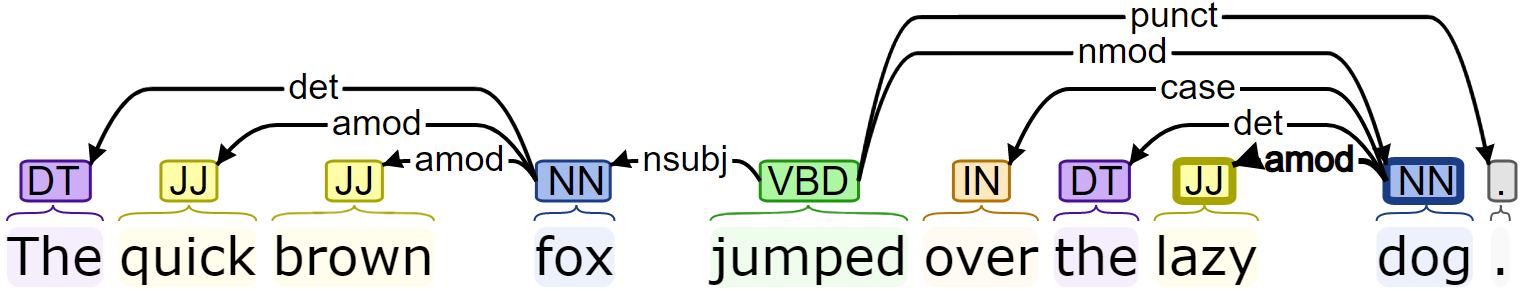
\includegraphics[width=\linewidth]{reports/technical_report/latex/figures/dependency_parse.png}
    \caption{An example of a dependency parse.\protect\footnotemark 
    For a description of what the relations on the arcs mean refer to page 3 of \citep{martin2009speech}.}
    \label{fig:dependency_parse_example}
\end{figure}

\footnotetext{
    Figure generated from \url{https://corenlp.run/}.
}

\subsection{Edges \& Relating Concepts}
In the graph structure we are building a relationship between concepts is represented as a directed edge between nodes. Edges are used to represent a `references' type relationship between concepts. The scheme I choose for relating two concepts has two main criteria: an edge is created from the subject of the sentence to any other concepts in the same sentence; an edge is created between any `complex' concept and each of the constituent concepts extracted from the complex concept. So how do we identify the subject of a sentence? We can do this through a dependency parse, which marks the relationships between words in a sentence. See Figure \ref{fig:dependency_parse_example} for an example. 

\begin{figure}
    \centering
    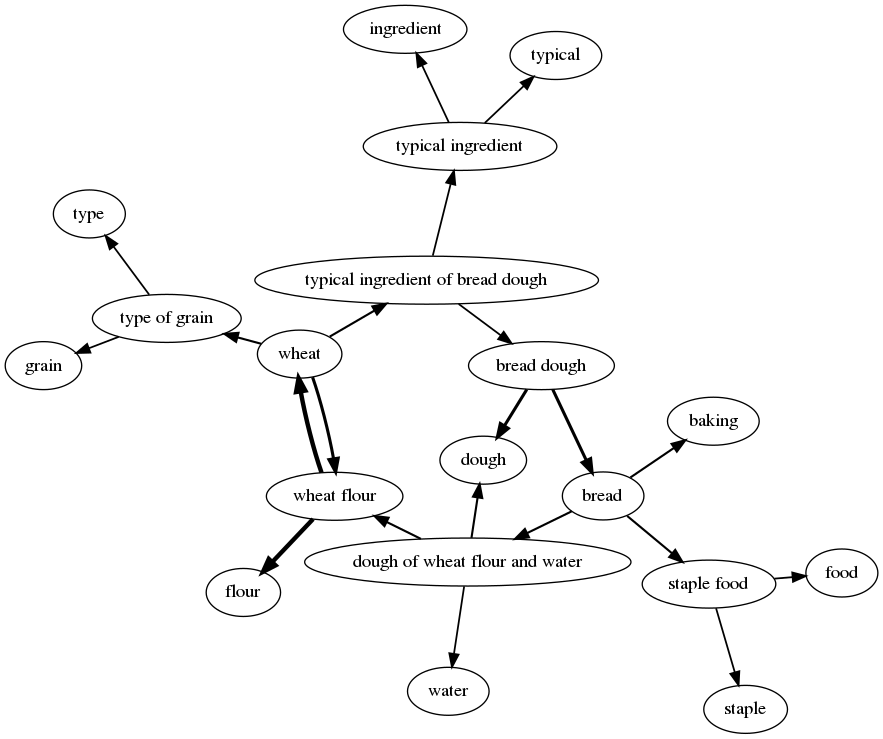
\includegraphics[width=\linewidth]{reports/technical_report/latex/figures/bread_graph-sections_only-implicit_references.png}
    \caption{An example of a dependency-based graph created using the XML document from Figure \ref{fig:sample_xml_document}. Nodes represent the concepts that are referenced in the document. Edges in the graph represent the relationship `A references B'. Blue edges represent forward references and red edges represent backward references.}
    \label{fig:graph_example}
\end{figure}

\subsection{Summary}
By using part of speech tags and a regex-based chunker we can extract concepts from text. At present concepts are only defined in a limited scope (mainly just nouns). We can derive relationships between concepts by looking at dependency parses of sentence structures and by looking at the constituent parts of complex concepts represented by compound nouns. Concepts are represented as a node in the graph and relationships between concepts are represented as edges in the graph.

\section{Graph Analysis} \label{sec:graph analysis}
In this section I will discuss how different types of concepts and references can be identified in a graph, and then how we can derive a score of conceptual density from the graph.

\subsection{A Priori \& Emerging Concepts}
A priori and emerging concepts can be identified in a graph by looking at the incoming edges. For a given node, we can look at each of the edges associated with that node. If all of the incoming edges come from nodes in the same section as the node in question, then we can say that the node represents an a priori concept. Otherwise, if there are two or more sections that the incoming edges originate from, then we can say that the node in question represents an emerging concept.

\subsection{Forward and Backward References}
In the section-centric graph, forward and backward references can be found through a DFS (depth-first search) and identifying when the algorithm crosses between sections (see Algorithm \ref{alg:mark edges}). A prerequisite is that we must record the sections that appear in the text, and the order in which they are introduced during the parsing of the text document. Then, we can perform a DFS originating from the nodes that represent the main concept of the sections. We can identify a forward reference when the DFS algorithm visits a node that is associated with a section that comes after the section of the previously visited node. Similarly, backward references can be identified when the DFS algorithm visits a node that is associated with a section that comes before the section of the previously visited node. When the algorithm crosses between sections the edges between the current and previous node can then be appropriately marked as a forward or backward reference. An example of a graph where the forward and backward egdes have been coloured is shown in Figure \ref{fig:graph_example-coloured_edges}.

\SetKwProg{Fn}{Function}{}{end}
\SetKwFunction{FMarkEdges}{markEdges}
\DontPrintSemicolon

\begin{algorithm*}
    \caption{Marking Forward and Backward References}
    \label{alg:mark edges}
    \KwData{
        $sections$: List of sections in a given document $D$ \\
        $nodes$: Set of nodes in the graph $G$ \\
        $adj$: Adjacency list for a directed graph $G$.\\
    }
    \;
    $visited = \emptyset$\;
    \;
    \For{$node \in$ nodes}{
        markEdges($node$, NULL, visited)\;
    }
    \;
    \Fn{\FMarkEdges{curr, prev, visited}}{
        \tcc{
            Arguments\\
            curr: Current node\\
            prev: Previous node\\
            visited: Set of visited nodes
        }
        \;
        \uIf{$prev \neq NULL$ AND $curr.section \neq prev.section$}{
            $curr\_i \gets sections.indexOf(curr.section)$\;
            $prev\_i \gets sections.indexOf(prev.section)$\;
            \;
            \uIf{$curr\_i < prev\_i$}{
                Mark edge $\{prev, curr\}$ as a backward reference\;
            }
            \uElseIf{$curr\_i > prev\_i$}{
                Mark edge $\{prev, curr\}$ as a forward reference\;
            }
        } 
        \uElseIf{$curr \notin visited$}{
            $visited \gets visited \cup \{curr\}$\;
            \;
            \For{neighbour $\in$ adj[curr]}{
                markEdges(\textit{neighbour, curr, visited})\;
            }
        }
    }
\end{algorithm*}

% \subsection{Cycles} 
% We can also consider the number and length of cycles in the graph. Cycles in a graph would suggest the existence of self-referential loops in the text document - in other words sets of concepts that are defined in terms of themselves. Long cycles are perhaps not of too much concern since a long cycle may not necessarily encode a strong dependency between all of the concepts in the cycle. Short cycles, on the other hand may be indicative of strong interdependence and may prove difficult to learn the corresponding concepts since learning one of the concepts in isolation may not suffice.

% \subsection{Isolated and Disjoint Subgraphs} 
% The idea of identifying bottlenecks in the graph structure can be extended to finding subgraphs that form isolated/disjointed clusters. Isolated clusters would be a set of interconnected vertices that have a small number of edges connecting them to the rest of the graph. These clusters would likely represent areas of a knowledge domain that could be learned in relative isolation from the reset of the domain, as long as the bottleneck concepts are learned. Similarly, disjointed subgraphs would also denote a similar thing. The existence of these isolated clusters or disjointed subgraphs would imply lower conceptual density than the alternative - a highly interconnteced graph.

\begin{figure}
    \centering
    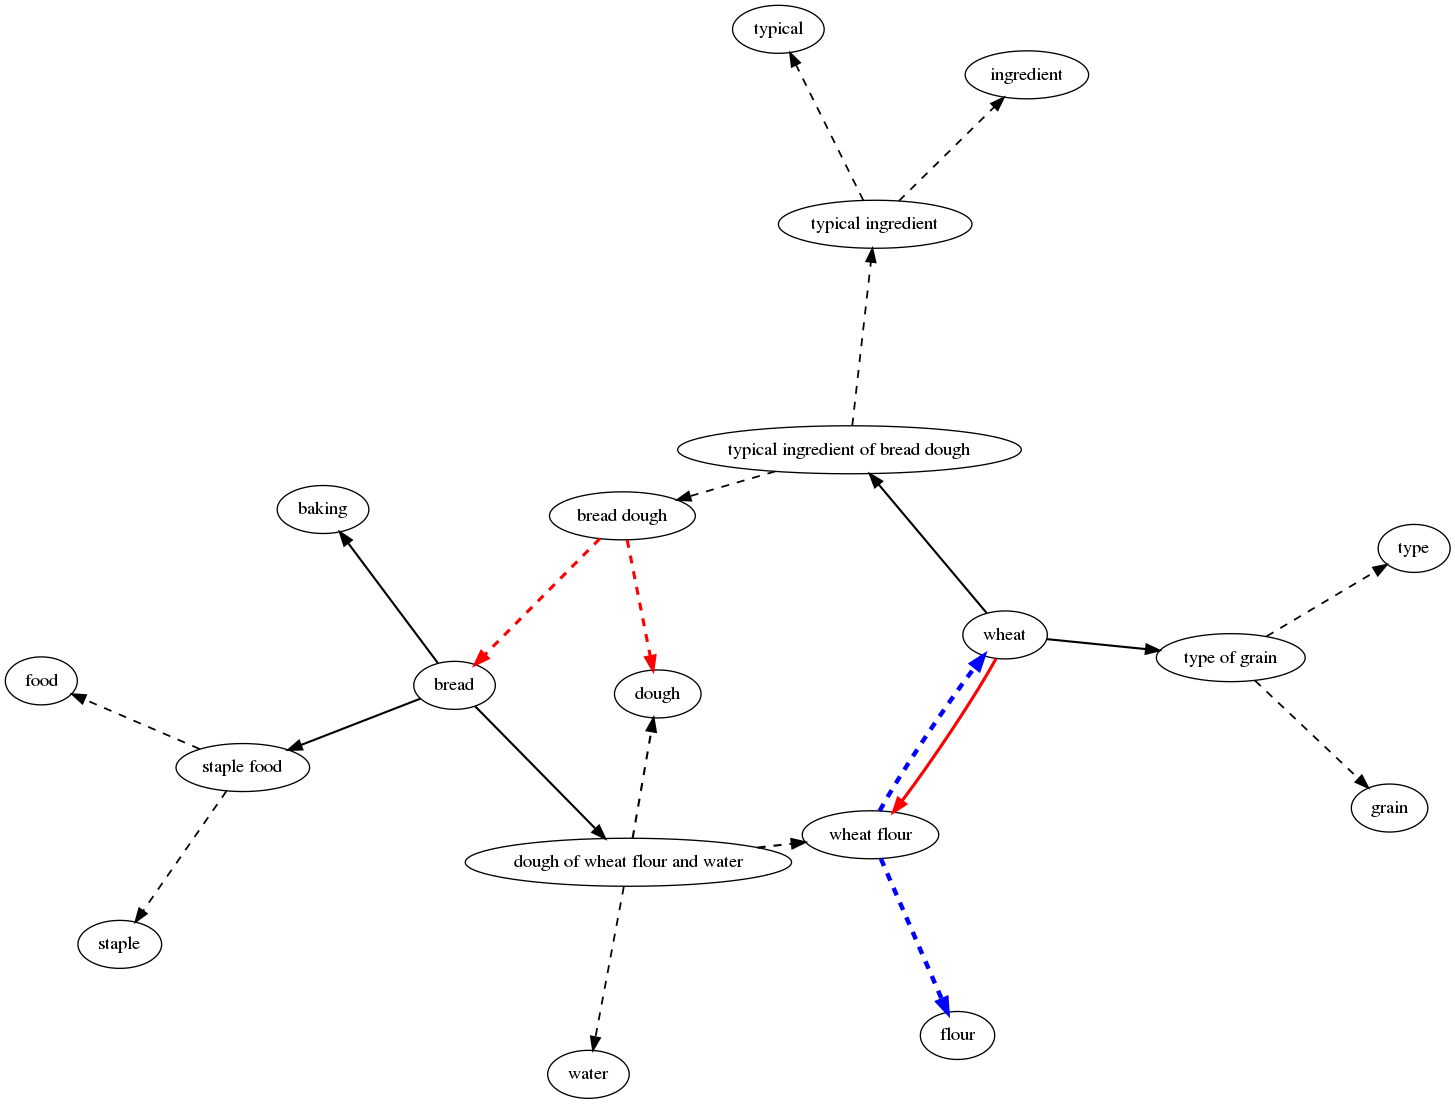
\includegraphics[width=\linewidth]{reports/technical_report/latex/figures/bread_graph-sections_only.png}
    \caption{An example of a dependency-based graph created using the XML document from Figure \ref{fig:sample_xml_document} where forward and backward references have been coloured. Nodes represent the concepts that are referenced in the document. Edges in the graph represent the relationship `A references B'. Blue edges represent forward references and red edges represent backward references.}
    \label{fig:graph_example-coloured_edges}
\end{figure}

\subsection{Quantifying Conceptual Density} \label{sec:quantifying_conceptual_density}
At the centre of conceptual density is the notion of the degree of integration between concepts. In the graph structure this can be measured by looking at the connectivity of nodes. One useful measure may be the average outdegree:
\begin{equation} \label{eq:simple score}
    S_D = \frac{1}{|V|} \sum_{v \in V} \text{deg}^+(v)
\end{equation}
where $S_D$ is the score of the document $D$, $V$ is the set of vertices in the graph,  and $\text{deg}^+(v)$ is the outdegree, or the number of outgoing edges from the vertex $v$. The interpretation of a high average degree can be either: the concept is related to many other concepts and therefore harder to learn since you must learn the other concepts as well; or the concept is related to many other concepts and therefore easier to learn since you have more knowledge to which you can relate the concept. I choose the former interpretation. 

% Perhaps it is not appropriate to include the number of vertices into the score. After all, the main contributor to conceptual density is not necessarily the number of concepts, but rather the interaction between the concepts and the degree to which the concepts interact. Going back to the element interactivity effect, again we are simply concerned with the number of \textit{interacting} elements. There is bound to be correlation between the number of vertices and the average outdegree, so perhaps information about the number of vertices in the graph is implicitly, and partially, encoded in the measure of average (out)degree. Furthermore, including the number of vertices into the score may lead to bias to longer documents. Longer documents have more opportunities to elaborate and give examples compared to shorter documents. And whether or not a longer document is more conceptually dense than a shorter document should be based on the interactions of the concepts. Thus, I believe that it is best to leave out the number of vertices from the scoring metric, thus reducing the score to:
% \begin{equation} \label{eq:simple score without vertices}
%     S_D = \frac{1}{|V|} \sum_{v \in V} \text{deg}^+(v)
% \end{equation}

% We can further refine the scoring method by taking into account the strength of the edges, or in other words the weights of the edges:
% \begin{equation} \label{eq:weighed score}
%     S_D = \frac{1}{|V|} \sum_{v \in V} \sum_{w \in W_v} w
% \end{equation}
% where $W_v$ is the set of weights for the outgoing edges of the vertex $v$, and $w$ is a single weight for a given edge. The previous formulation in Equation \ref{eq:simple score} can be thought of as a special case of this formulation where the weight for every edge is one.
% The weight for given edge can be adjusted based on the type of reference the edge represents. For example, we could set the weight of an edge to: 0.5 for implicit references since they are not explicitly represented in the text and as such the reader may not need consider the referenced concept; 1.0 for references to a priori concepts since they typically represent a concept that the reader is expected to know beforehand and only impose germane load; 1.5 for backward references since the reader is required to recall a concept that may have been introduced within the text and using a poorly integrated schema will require more mental exertion than when considering an a priori concept; and 2.0 for forward references since the reader is required to \textit{park} a new concept without anything concrete to pin it too, increasing cognitive load. The exact numbers are not important, but rather the relative scales of the numbers. references to a priori concepts should impose less cognitive load than backward references, and backward references should impose less cognitive load than forward references.

% What about references that occur often? If concept A references concept B 100 times, and concept C references concept D 10 times, out of the referenced concepts B and D which would be more difficult to learn? Perhaps a concept being referenced frequently means there are plenty of examples to learn concept B, making it relatively easy to learn concept B. On the other hand, infrequent references to a concept may indicate that the concept is mentioned in passing or as an example and that the concept is relatively simple. Maybe just looking at the frequency of references does not give us enough information to decide this. In this report I will use the interpretation that highly frequent references indicate a higher level of interdependence between two concepts, and as such higher conceptual density. I choose to incorporate frequency into the score by taking a weighted frequency:
% \begin{equation} \label{eq:weighed frequency score}
%     S_D = \frac{1}{|V|} \sum_{\{x, y\} \in E} w(x, y) f(x, y)
% \end{equation}
% where $E$ is the set of all edges $\{x, y\} $ in the graph, $w: \{x, y\} \mapsto \mathbb{R}^+$ is a function that maps the edge $\{x, y\}$ to a weight, and $f: \{x, y\} \mapsto \mathbb{Z}^+$ is a function that maps the edge $\{x, y\}$ to a frequency count.

% One possible issue with Equation \ref{eq:weighed frequency score} is that a reference with a frequency of 40 is not necessarily much more important than a reference with a frequency of 20. In extreme cases, how important is the frequency of a reference when we get to frequency counts of  100 and 200. There is a point where a higher frequency does not really mean much. Thus, it may be sensible to scale down large frequency counts. I do this by scaling the weighted frequency logarithmically: \todo{what is the precedent for this? (Zipf's law, typical language models, tf-idf?)}
% \begin{equation} \label{eq:log weighed frequency score}
%     S_D = \frac{1}{|V|} \sum_{\{x, y\} \in E} 1 + \text{log}_2 (1 + w(x, y) f(x, y))
% \end{equation}
% where I add one to the argument to the log function so that the most basic reference (weight of one, frequency of one) results in zero, in other words no effect. Adding one to the logarithmically-scaled weighted frequency means that the minimum contribution of an edge to the score is one.

% However, as discussed in Section \ref{sec:presentation of concepts} not all references are created equal. So the type of reference should be taken into account. This is done by assigning different weights to the different types of references. We can also include the frequency of references (e.g. how often A references B) and combine it with the associated weights. I also scale this weighted frequency logarithmically in case a single or few concepts are dominant in a text. For example, in this paper words such `concept' and `graph' appear in almost every section and mentioned frequently. These types of dominant concepts may skew the score of an otherwise simple document and so I scale the frequency count of references.

% Including cycles and disjointed subgraphs, we can define a scoring scheme of conceptual density for a given document as such:
% \begin{equation*}
% 	\begin{aligned}	
%     S_D =\ &|C| + \frac{1}{|C|} \sum_{c \in C} |c| \\ 
%     			&+ |M| + \frac{1}{|M|} \sum_{m \in M} |m| \\
%     			&+  \frac{1}{|V|} \sum_{\{x, y\} \in E} 1 + \text{log}_2 (1 + w(x, y) f(x, y))
% 	\end{aligned}
% \end{equation*}
% where $S_D$ is the score for a given text document $D$, $C$ is the set of simple cycles in the graph, $c$ is a simple cycle in $C$, $M$ is the set of disjointed subgraphs in the graph, $m$ is a disjointed subgraph in $M$, $V$ is the set of all vertices (nodes) in the graph, $E$ is the set of all edges $\{x, y\} $ in the graph, $w: \{x, y\} \mapsto \mathbb{R}^+$ is a function that maps the edge $\{x, y\}$ to a weight, and $f: \{x, y\} \mapsto \mathbb{Z}^+$ is a function that maps the edge $\{x, y\}$ to a frequency count.
%  I add one to the argument to the log function so that the most basic reference (weight of one, frequency of one) results in zero, in other words no effect. Adding one to the log term means that the minimum contribution of an edge to the score is one.

\section{Related Work} \label{sec:related_work}
% \subsection{The  PMOSE/IKIRSCH  document readability  formula?}
% This paper \citep{mosenthal1998new}
% \begin{itemize}
%     \item A measure of document complexity
%     \item Only takes into account layout/structure and reference to external information
% \end{itemize}

% \subsection{Automatic Essay Grading?}

\subsection{Information Extraction}
The process of identifying concepts and how they are related that I have described in this report is similar to the task of information extraction. However, there are some key differences between what I have done and what is usually done in information extraction. First and foremost, information extraction is typically concerned with named-entity recognition - the identification of named-entities such as names of people, companies, locations, and dates. In this project we are concerned with concepts in general (all types of entities), which can be thought of as a superset of named-entities. Furthermore, information extraction is also interested in the relationship between named-entities. However, in this project and the work-to-date we are not too concerned about the nature of a relationship between concepts as much as we are interested in just the existence of a relationship.

\subsection{Semantic Networks \& Knowledge Graphs}
The type of graph structure that is being built up in this project is very similar to semantic networks and knowledge graphs. Some differences between the graphs in this project and semantic networks are that: we are not annotating edges with the type of relationship (e.g. X IS\_A Y or X HAS\_A Y), and the criteria for deciding what constitutes a node or edge in the graph may differ from what is common in the literature. \todo{How so?}

\section{Future Work} \label{sec:future_work}
\subsection{Transitioning to Unstructured Text}
I have implemented a section-centric graph from semi-structured text (e.g. Figure \ref{fig:graph_example}), but recreating the same graph from the corresponding plain text version of a document remains difficult. I have discussed some challenges that may arise when building a section-centric graph from unstructured text. A combination of topic segmentation methods and natural language processing techniques to identify topics may enable the creation of such a graph from unstructured text. The quality of the extracted relationships between concepts can also be improved through the use of dependency trees.

Another issue with semi-structured text is that it requires someone to manually mark up the text. Having an implementation that can work with unstructured text would remove the need to do this and allow for much easier use.

\subsection{Improving Information Extraction}
One issue with the current work is the quality of the extracted concepts and how the concepts are related. There are many cases where the extracted concepts do not align with the concepts that a human would intuitively pick out, and similarly for how concepts are related. While the current quality is adequate enough to build up a graph structure, important concepts and relationships between concepts are likely to be missed. So it is important that future work focuses on improving the quality of extracted concepts and relations.

\subsubsection{Extending the Definition of a Concept in Text}
In addition to noun phrases we can include other types of phrases into the definition of a `concept'. We can extend the definition of noun phrases to include two noun phrases joined by a preposition. For example, consider the phrase ``relationships between concepts''. Under the previous definition we would consider ``relationships'' and ``concepts'' as two separate noun phrases, however it is equally sensible to consider the entire phrase as a single entity. We can also include particular types of verb phrases. For example, consider the sentence ``Listening to music is his favourite way to pass time'', what are the concepts being talked about here? I believe it would be sensible to say that the concepts of ``listening to music'' and ``passing time'' are being discussed. Adding these types of phrases leads to a more rich definition of a `concept'. 

\subsubsection{Better Dependency Parsing}
The current scheme for relating concepts in the dependency-based graph simply relates the subject of a sentence to the other concepts that appear in the sentence. This does not capture the nuances of natural language very well. For example, consider the sentence ``Wheat is used for making wheat flour, a typical ingredient of bread dough'' from Figure \ref{fig:sample_txt_document}. Under the current scheme the subject, `Wheat', would have an edge created between itself and the other concepts `wheat flour' and `typical ingredient of bread dough'. However, the sentence is phrased such that wheat flour is being to referred to as a `typical ingredient of bread dough', not `wheat'. A more correct set of edges in this case would connect `wheat' to `wheat flour' and `wheat flour' to `typical ingredient of bread dough'. 

\subsubsection{Information Extraction Frameworks} Much of the work in this project has been inspired by other work but built from scratch. As discussed earlier, much of the process of extracting and relating concepts is similar to the task of information extraction. There exists a framework called OpenIE \citep{banko2007open} which is made for performing information extraction. The benefits of using such a framework is that many of the issues with the current dependency parsing in this project have more or less been solved in OpenIE. A couple of issues that I foresee with adapting a framework such as OpenIE to use in this project are that OpenIE is geared towards working with named-entities and it may be difficult to recover section information relating to extracted entities. 
% Perhaps there are patterns in the dependency parse that could be used to assign the correct relation in this sort of case.
%In this particular case, `wheat flour' is the direct object of `making' and `typical ingredient` is the appositive modifier of `wheat flour'.


\subsection{Other Graph Features}
There are many graph analysis techniques that have not been explored in this report (see \citep{algorithms_documentation}, for example). It would be interesting to see if incorporating features derived from these analysis techniques into the scoring scheme improves the quality of it.

\subsubsection{Bottlenecks} \label{sec:bottlenecks}
Another interesting possible feature in the graph topology is the idea of a bottleneck vertex/vertices that might be able to be found by identifying the minimum cuts of the graph. One could imagine a bottleneck in a graph structure being visually similar to a hourglass.
% (see Figure \ref{fig:bottleneck example} in  \ref{sec:supplementary figures} for an example).
The vertex at the centre of the hourglass shape would be the bottleneck vertex. This would correspond to a concept that is defined in terms of other concepts and is used to define a set of other concepts. For example, in programming polymorphism and inheritance cannot be explained if classes are not explained, similarly classes cannot be explained if variables and functions are not explained. While in this example we could imagine back references from polymorphism to functions, to explain polymorphism we must first explain classes. Therefore, directionality must included when defining and identifying bottleneck concepts. Bottleneck concepts are important to the idea of conceptual density because they make learning more difficult.

\subsubsection{A priori concepts}
It may be possible to redefine what an a priori concept is in terms of sinks in a graph. A sink is a node in a directed graph that has an outdegree of zero, i.e. it has no outgoing edges. Identifying sinks in a graph is trivial, but we could also extend the idea of an a priori concept being a concept that is only referenced from within one section to: a concept that only leads to a sink and is not part of a self-referential system. 

\subsection{Other Text Features}
There are other features that could be extracted from text.
In \citep{robins2010learning} it is suggested that a measure of distance between keywords (concepts) could be used to help measure conceptual density. There are some methods that may help with this such as: using lexical chains for keyword extraction \citep{ercan2007using}; and looking at long distance dependency as a metric of reading comprehension difficulty \citep{liu2008dependency}. 

\subsection{Evaluation of the Scoring Scheme} \label{sec:evaluation_of_the_model}
Regarding the evaluation of the scoring algorithm, the quality of the scores derived from graphs that were generated from semi-structured text have only been evaluated qualitatively in an ad-hoc manner. One particular experiment that I envision is one performed on a labelled data set of abstracts created from human judgements. We need to use human judgements since, as discussed near the start of this report, there no objective measures of conceptual density or element interactivity and as such human judgements are the only baseline available to compare the model with. For the collection of documents, we could gather a number of snippets from various textbooks that consist of a few sections. The reason for choosing snippets that contain is that they are short, self-contained, expository documents. And if we are to get human judgements then it will be a lot easier and a lot less time consuming to use abstracts as apposed to long documents such as textbooks. Once a collection of abstracts have been created we could group abstracts into pairs and get a panel of human judges to judge which document appears to be more conceptually dense.  Then, we could compare the output of the model against the human judgements and see how well it mimics the human judgements.

\subsection{Feature Importance Analysis}
From the process described in Section \ref{sec:evaluation_of_the_model} we would create a labelled data set. From this we could train a machine learning algorithm such as a simple linear regression or random forest. Then through feature importance analysis we could investigate which features out of all of the extracted features (from text and the graph structure) are the most salient in regards to conceptual density. And with a large enough data set, we could simply extract as many features as possible, regardless of whether or not they seem relevant to conceptual density, and then use this feature importance analysis to filter out the unimportant features in a principled way.

\section{Conclusion} \label{sec:conclusion}
In this report I have explored a graph-based approach to quantifying conceptual density - an idea relating to the degree that concepts of a particular knowledge domain, encoded by a text document, are integrated. I have discussed how this idea of conceptual density is grounded in, and related to, learning edge momentum and cognitive load theory. I have discussed the ways in which the notion of conceptual density can be defined and measured in semi-structured and unstructured text documents. By analysing the language in the documents and observing the patterns in natural language we can create an operational definition of a `concept' in text. Then by analysing the relationships between concepts in a given document we can build up a graph structure from which we can derive a score of conceptual density. 


% \bibliographystyle{acm}
\bibliography{report}


% % Activate the appendix
% % from now on sections are numerated with capital letters
% \appendix

% % \renewcommand{\thesection}{Appendix \Alph{section}}

% \section{Implementation Details}
% \begin{itemize}
%     \item Parsing Unstructured Text
    
%     \begin{itemize}
%         \item Normalisation Techniques
%         \item Sentence and Word Tokenisation
%         \item POS Tagging
%         \item Regex Chunking
%         \item Constituency Trees
%     \end{itemize}
% \end{itemize}

% \subsection{Relevant NLP Methods?}
% \begin{itemize}
%     \item Parts of Speech Tagging
%     \item Constituency Parsing/Chunking
%     \item Dependency Parsing
% \end{itemize}

% \subsection{Relevant Graph Analysis Techniques?}
% \begin{itemize}
%     \item Minimum cut
% \end{itemize}

% % \section{Synthesised Text Corpus}
% % We created a small corpus of hand-crafted text documents. These can be separated into three main groups: one group where the text is as simple as possible and is minimally conceptually dense; one group where ideas are dependent on the ones preceding it; and one final group where an attempt was made to make the most entangled mess possible. The idea is that each of these groups of texts will have characteristics that we believe will lead to low, medium, and high conceptual density respectively, purposefully inserted.

% \section{Supplementary Figures} \label{sec:supplementary figures}

% \begin{sidewaysfigure}
%     \centering
%     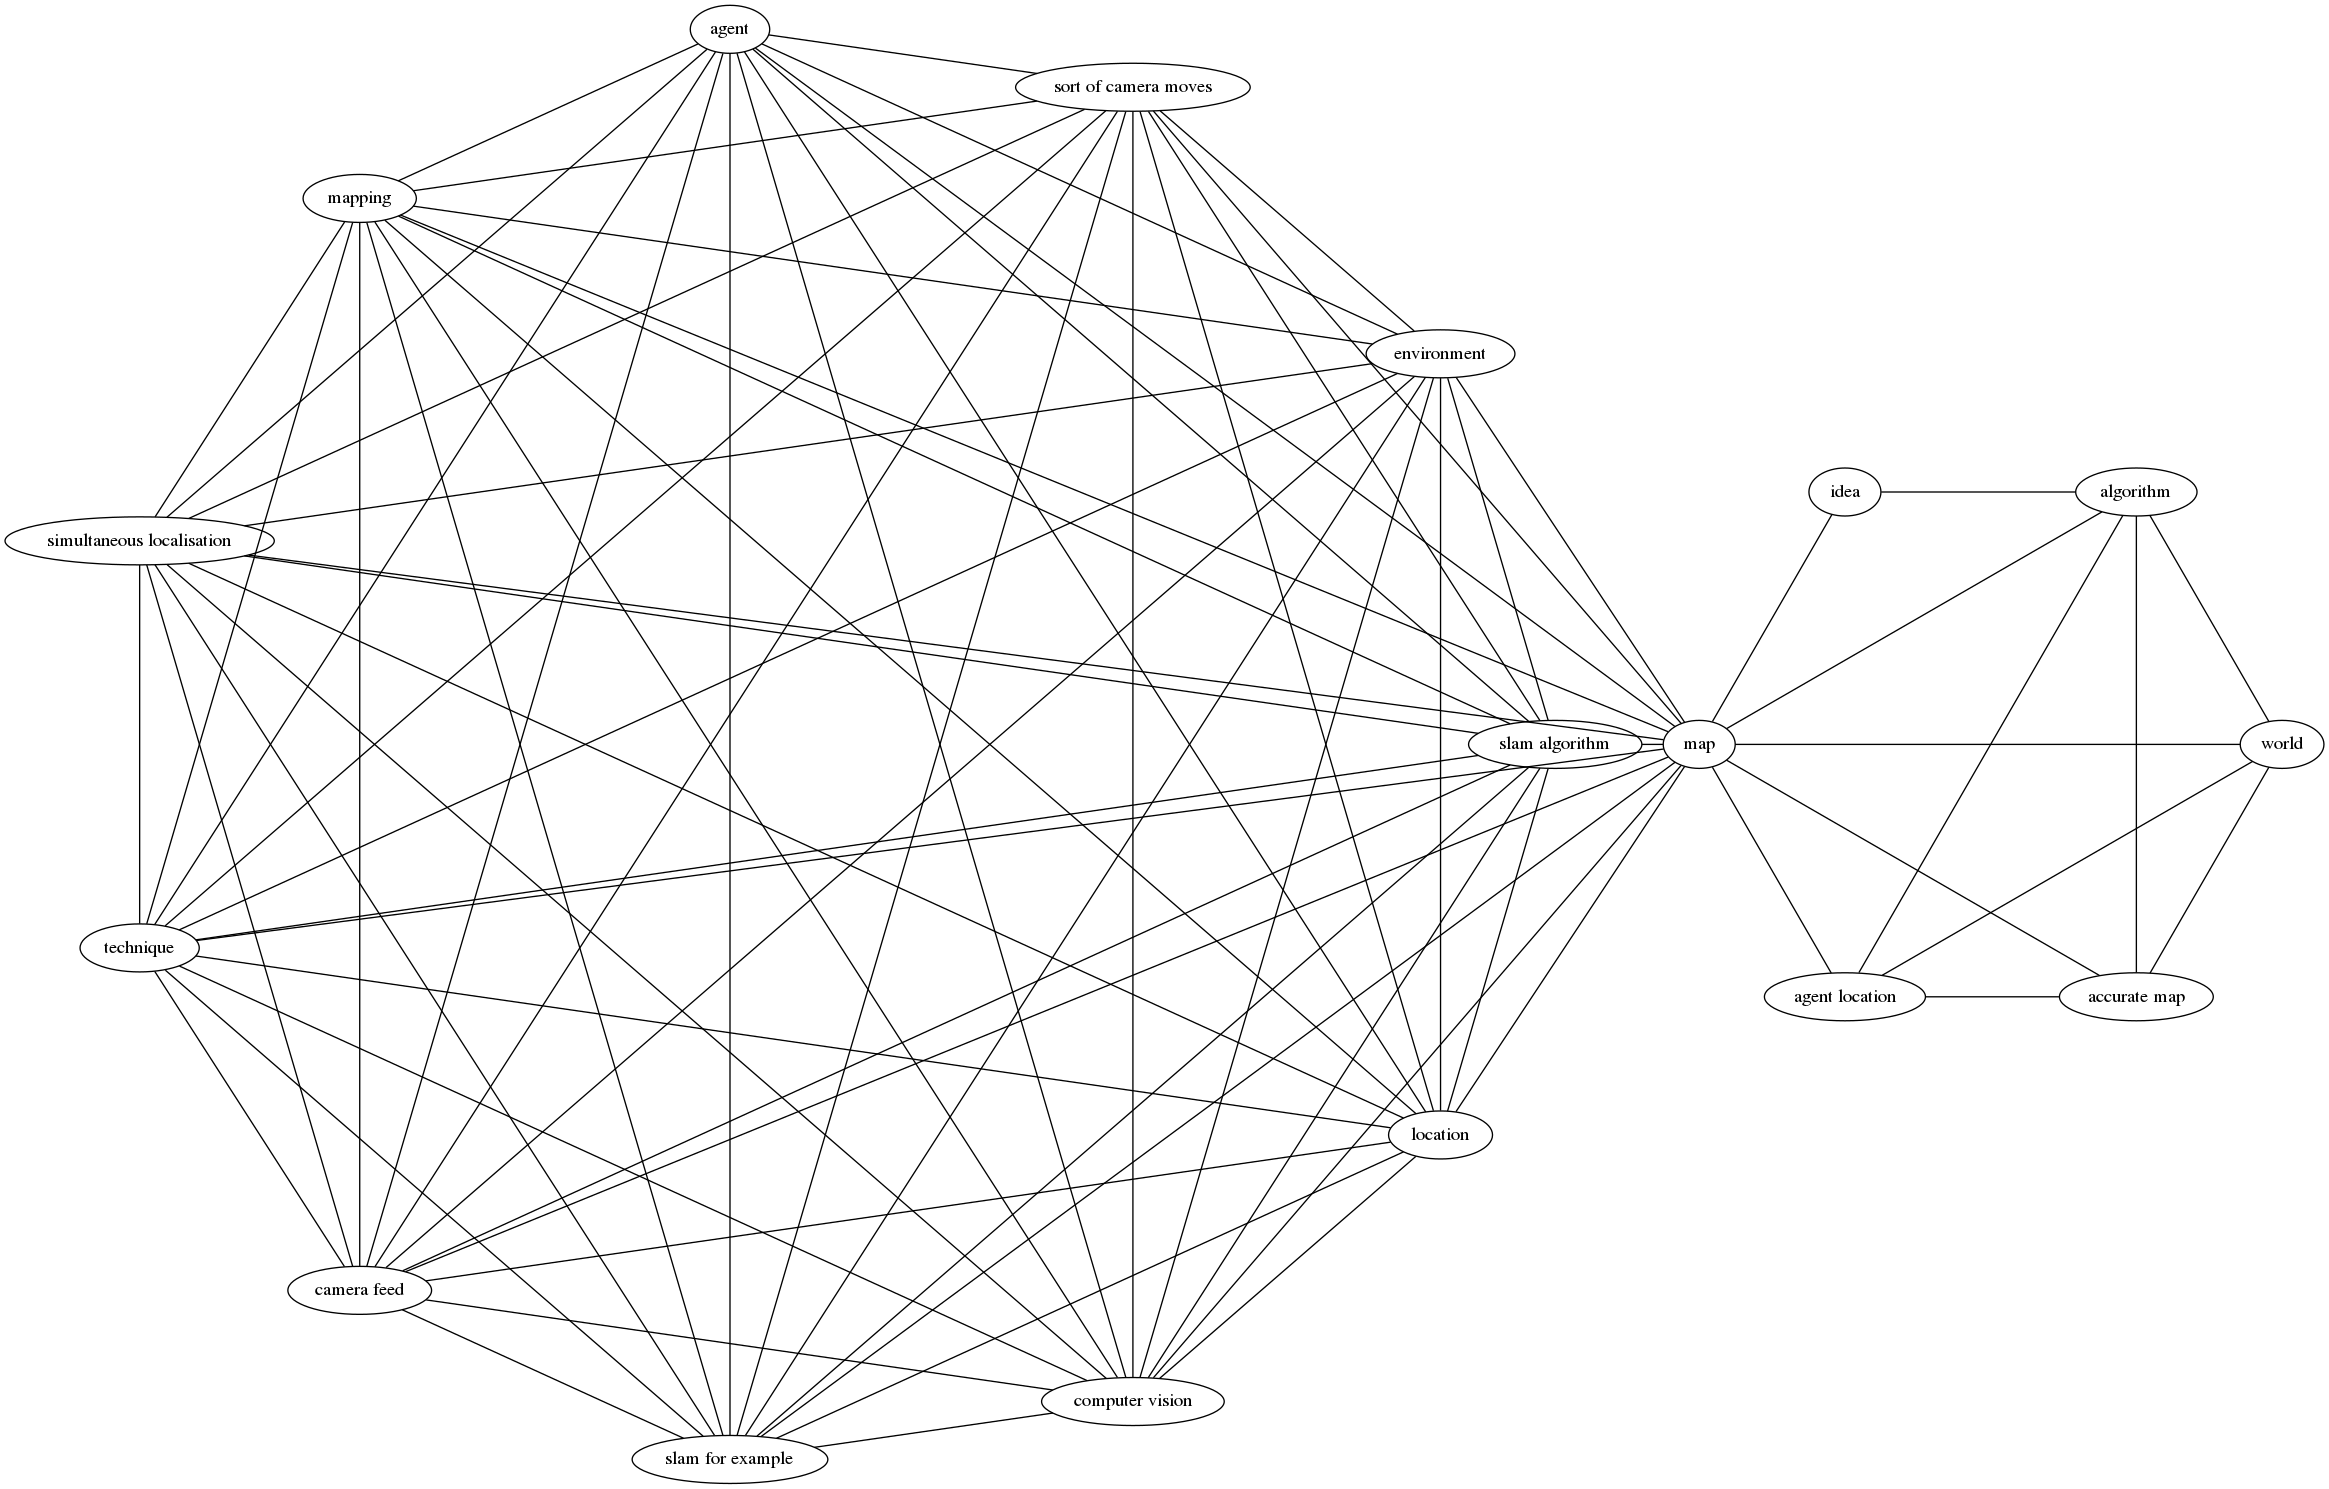
\includegraphics[width=\linewidth]{reports/technical_report/latex/figures/bottleneck.png}
%     \caption{An example of a graph built from unstructured text using simple co-occurrence. Notice that the graph is densely connected, and that it also forms the sort of hourglass structure mentioned in Section \ref{sec:bottlenecks}}
%     \label{fig:bottleneck example}
% \end{sidewaysfigure}

\end{document}